\chapter{Power consumption}
In this chapter are presented the calculations performed for the power consumption in CMOS multiplexers. By using the application TAMTAMS web, it was possible to make a first analysis at system level of several parameters concerning CMOS NAND2 gates employed.  
\section{Theoretical analysis}
\paragraph{Static Power}
is generated by the contribution of two different leakage currents: subthreshold current and gate current.
Static power is considered as the product between the supply voltage $\left( V_{dd} \right)$  and the leakage currents probabilistic mean value.
\\
\paragraph{Dynamic Power}
is described by the following expression
\begin{equation*}
P_{DYN}= f_{ck} V_{DD}^{2} E_{SW} C_{L},
\end{equation*}
where contributes are:
	\begin{description}
		\item[$V_{DD}$] voltage supply. Dynamic power consumption has a quadratic relation with it, so to reach a further power dissipation decreasing we should act on it;
		\item[$f_{ck}$] clock frequency. Faster is the device behaviour, higher is the consumption;
		\item[$E_{SW}$] switching activity. It is the number of transition per period;
		\item[$C_{L}$] load capacitance. Is the load that the device has to drive.
	\end{description}
To compute the dynamic power consumption, the basic MUX unit has been studied and the worst case has been selected: the maximum switching activity has been obtained analyzing the following truth table where the starting configuration is assumed as $A=B=0$ and $S=1$:
	\begin{table}[h]
	\centering
	\caption{Truth table for transition analysis}
	\label{my-label}
		\begin{tabular}{lllll}
		\textbf{A} & \textbf{B} & \textbf{S} & \textbf{Y} & \textbf{Transitions} \\
		0          & 0          & 0          & 0          & 1                    \\
		0          & 0          & 1          & 0          & 0                    \\
		0          & 1          & 0          & 0          & 2                    \\
		0          & 1          & 1          & 1          & 2                    \\
		1          & 0          & 0          & 1          & 3                    \\
		1          & 0          & 1          & 0          & 0                    \\
		1          & 1          & 0          & 1          & 3                    \\
		1          & 1          & 1          & 1          & 2                   
		\end{tabular}
	\end{table}

%%TODOOOOOOOOOOOOOOOOOOOOOOOOOOOOOOOOOOOOOOOOOOOOOOOOOOOOOOOOOOOOOOOOOOOOOOO	

We have maximum switching activity when $A=1$, $B$ doesn't care, $S=0$. This configuration determines that three gates (2 NAND2 and 1 inverter) output commute at the same time (see figure \ref{fig:2_to_1_1bit_dyn}). 
In order to compute the dynamic power consumption we have taken into account only the worst case condition, considering for every elementary mux structure the consumption associated to the commutation of 2 NAND2 and 1 inverter.
	\begin{figure}[h]
		\centering
		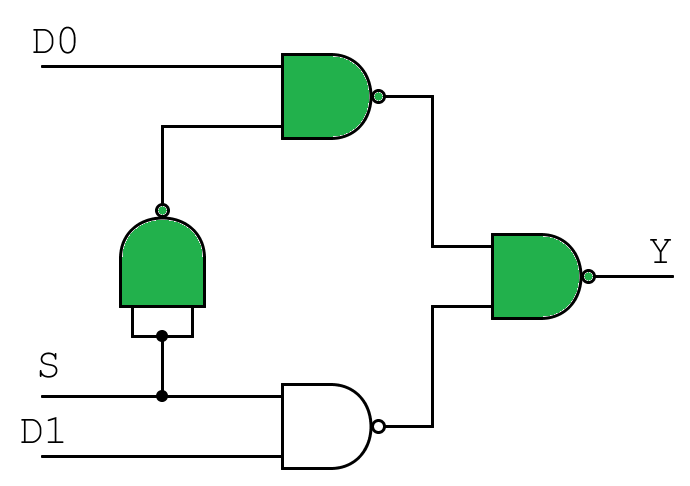
\includegraphics[width=0.5\textwidth]{immagini/2_to_1_1bit_dyn.png}
		\caption{Basic MUX structure. In green are represented gates defining the maximum switching activity.}
		\label{fig:2_to_1_1bit_dyn}
	\end{figure}
%---------------------------------------------------------------
%	MODELLI
%---------------------------------------------------------------
\subsection{Models}
Here is presented the models employed in the power evaluation. To represent the characteristics of each mux circuit, we used the following notation:  
	\begin{description}
		\item[$X$]	stands for configuration number input;	%numero di input della configurazione
		\item[$W$]	describes the parallelism, number of bit, that compose a single mux input information.
	\end{description}
\paragraph{Static power model}
To compute the total amount of static power, it is necessary to consider the single NAND2 static power consumption, obtained with TAMTAMS analysis. This value has to be multiplied by the total number of gates in the configuration under exam. For instance,a basic 2-to-1 mux with $W=1$, is obtained from a total amount of 4 NAND2 gates  with fan out of 1 (FO1), according to figure \ref{fig:2_to_1_1bit_dyn}. Generalizing for a mux with number of input $X$ and parallelism $W$, it is possible to express a general equation describing the amount $N_{gates}$ of NAND2 needed.
\begin{equation}
N_{gates} = \underbrace{3 W \left( X-1 \right)}_\text{number of NAND2} \ \ \ \ \ \ \  + \underbrace{\frac{W}{4}\left( X-1\right) .}_\text{number of NAND2 to build inverters}
\label{magic}
\end{equation}
Moreover, the term expressing the number of NAND inverter, gives information about the fan-out of inverters in the circuit. Let's see three examples of how this equation work.
\textbf{Example 1}\\
Consider a mux 4-to-1 with W=2.\\
The amount of logic NAND2 needed are:  $3 W \left( X-1 \right) = 18. $
The amount of NAND2 inverters are: $W/4\left( X-1\right) = 1.5=  \underbrace{1}_\text{one NAND2 FO4} + \underbrace{0.5}_\text{one NAND2 FO2}$\\
\textbf{Example 2}\\
Consider a mux 8-to-1 with W=2.\\
The amount of logic NAND2 needed are:  $3 W \left( X-1 \right) = 42. $
The amount of NAND2 inverters are: $W/4\left( X-1\right) = 3.5=  \underbrace{3}_\text{tree NAND2 FO4} + \underbrace{0.5}_\text{one NAND2 FO2}$\\
\textbf{Example 3}\\
Consider a mux 8-to-1 with W=1.\\
The amount of logic NAND2 needed are:  $3 W \left( X-1 \right) = 21. $
The amount of NAND2 inverters are: $W/4\left( X-1\right) = 1.75=  \underbrace{1}_\text{one NAND2 FO4} + \underbrace{0.5}_\text{one NAND2 FO2}+  \underbrace{0.25}_\text{one NAND2 FO1}$\\
In the end, to obtain the power values for static consumptions, numbers obtained with this model have been multiplied with the NAND2 static power dissipation values taken from TAMTAMS analysis.

\paragraph{Dynamic power model}
From considerations derived from the truth table with the analysis of transitions in a single 2-to-1 mux, presented at the beginning of this chapter, the mathematical expression representing maximum number of gate commutations in a generic X-to-1 mux with parallelism $W$ is 
\begin{equation}
N_{transitions} = \underbrace{2 W \left( X-1 \right)}_\text{wort case NAND2 transitions}   + \underbrace{\frac{W}{4}\left( X-1\right) .}_\text{wort case inverter transitions}
\end{equation}
As always, the term expressing the number of NAND inverter, gives information about the fan-out of inverters commuting in the circuit.
In order to  obtain the power values for the dynamic consumptions, numbers obtained with this model have been multiplied with the NAND2 dynamic power dissipation values taken from TAMTAMS analysis.
\newpage

\section{Simulation results}
\begin{table}[b!]
\centering
\label{my-label}
\begin{tabular}{@{}llllllll@{}}
\toprule
\multicolumn{2}{l}{\textbf{Configuration}} & \multicolumn{2}{l}{\textbf{HP\_2010}} & \multicolumn{2}{l}{\textbf{LOP\_2010}} & \multicolumn{2}{l}{\textbf{LSTP\_2010}} \\ \midrule
\textit{Input}         & \textit{Word}        & \textit{Static}   & \textit{Dynamic}  & \textit{Static}   & \textit{Dynamic}   & \textit{Static}    & \textit{Dynamic}   \\
2                      & 1                 & 0.00081W           & 7.133e-6W          & 8.076e-6 W         & 2.717e-6W           & 4.609e-7W           & 3.927e-6W          
\end{tabular}
\end{table}

%2to1 Wx
% Please add the following required packages to your document preamble:
% \usepackage{booktabs}
\begin{table}[b!]
\centering

\label{my-label}
\begin{tabular}{@{}llllllll@{}}
\toprule
\multicolumn{2}{l}{\textbf{Configuration}} & \multicolumn{2}{l}{\textbf{HP\_2010}} & \multicolumn{2}{l}{\textbf{LOP\_2010}} & \multicolumn{2}{l}{\textbf{LSTP\_2010}} \\ \midrule
\textit{Input}         & \textit{Word}        & \textit{Static}   & \textit{Dynamic}  & \textit{Static}   & \textit{Dynamic}   & \textit{Static}    & \textit{Dynamic}   \\
2                      & 8                 & 0.00524W           & 4.231e-5W          & 5.207e-5W          & 1.612e-5W           & 2.970e-6W          & 2.343e-5W           \\
2                      & 16                & 0.0105W            & 8.462e-5W          & 0.00010W           & 3.224e-5W           & 5.940e-6W           & 4.686e-5W           \\
2                      & 32                & 0.02097W           & 0.00017W           & 0.00021W           & 6.448e-5W           & 1.188e-5W           & 9.373e-5W           \\
2                      & 64                & 0.04194W          & 0.00034W           & 0.00042W           & 0.00013W            & 2.376e-5W           & 0.00019W           
\end{tabular}
\end{table}

%xto1 Wx
% input 16
\begin{table}[b!]
\centering
\label{my-label}
\begin{tabular}{@{}llllllll@{}}
\toprule
\multicolumn{2}{l}{\textbf{Configuration}} & \multicolumn{2}{l}{\textbf{HP\_2010}} & \multicolumn{2}{l}{\textbf{LOP\_2010}} & \multicolumn{2}{l}{\textbf{LSTP\_2010}} \\ \midrule
\textit{Input}         & \textit{Word}        & \textit{Static}   & \textit{Dynamic}  & \textit{Static}   & \textit{Dynamic}   & \textit{Static}    & \textit{Dynamic}   \\
16                     & 8                 & 0.0786W            & 0.0006W            & 0.0008W            & 0.0002W             & 4.455e-5W           & 0.0003W             \\
16                     & 16                & 0.1573W            & 0.0013W            & 0.0016W            & 0.0005W             & 8.9106e-5W          & 0.0007W             \\
16                     & 32                & 0.3145W            & 0.0025W            & 0.0031W            & 0.0010W             & 0.0002W             & 0.0014W             \\
16                     & 64                & 0.6290W            & 0.0051W            & 0.0062W            & 0.0019W             & 0.0004W             & 0.0028W            
\end{tabular}
\end{table}
% input 32
\begin{table}[b!]
\centering
\label{my-label}
\begin{tabular}{@{}llllllll@{}}
\toprule
\multicolumn{2}{l}{\textbf{Configuration}} & \multicolumn{2}{l}{\textbf{HP\_2010}} & \multicolumn{2}{l}{\textbf{LOP\_2010}} & \multicolumn{2}{l}{\textbf{LSTP\_2010}} \\ \midrule
\textit{Input}         & \textit{Word}        & \textit{Static}   & \textit{Dynamic}  & \textit{Static}   & \textit{Dynamic}   & \textit{Static}    & \textit{Dynamic}   \\
32                     & 8                 & 0.1625W            & 0.0013W            & 0.0016W            & 0.0005W             & 9.208e-5W           & 0.0007W             \\
32                     & 16                & 0.3250W            & 0.0026W            & 0.0032W            & 0.0010W             & 0.0002W             & 0.0015W             \\
32                     & 32                & 0.6500W            & 0.0052W            & 0.0065W            & 0.0020W             & 0.0004W             & 0.0029W             \\
32                     & 64                & 1.3000W            & 0.0105W            & 0.0129W            & 0.0040W             & 0.0007W             & 0.0058W            
\end{tabular}
\end{table}
% input 64
\begin{table}[b!]
\centering
\label{my-label}
\begin{tabular}{@{}llllllll@{}}
\toprule
\multicolumn{2}{l}{\textbf{Configuration}} & \multicolumn{2}{l}{\textbf{HP\_2010}} & \multicolumn{2}{l}{\textbf{LOP\_2010}} & \multicolumn{2}{l}{\textbf{LSTP\_2010}} \\ \midrule
\textit{Input}         & \textit{Word}        & \textit{Static}   & \textit{Dynamic}  & \textit{Static}   & \textit{Dynamic}   & \textit{Static}    & \textit{Dynamic}   \\
64                     & 8                 & 0.3302W            & 0.0027W            & 0.0033W            & 0.0010W             & 0.0002W             & 0.0015W             \\
64                     & 16                & 0.6605W            & 0.0053W            & 0.0066W            & 0.0020W             & 0.0004W             & 0.0029W             \\
64                     & 32                & 1.3210W            & 0.0107W            & 0.0131W            & 0.0041W             & 0.0007W             & 0.0059W             \\
64                     & 64                & 2.6420W            & 0.0213W            & 0.0262W            & 0.0081W             & 0.0015W             & 0.01181W           
\end{tabular}
\end{table}
% input 128

\begin{table}[b!]
\centering
\label{my-label}
\begin{tabular}{@{}llllllll@{}}
\toprule
\multicolumn{2}{l}{\textbf{Configuration}} & \multicolumn{2}{l}{\textbf{HP\_2010}} & \multicolumn{2}{l}{\textbf{LOP\_2010}} & \multicolumn{2}{l}{\textbf{LSTP\_2010}} \\ \midrule
\textit{Input}         & \textit{Word}        & \textit{Static}   & \textit{Dynamic}  & \textit{Static}   & \textit{Dynamic}   & \textit{Static}    & \textit{Dynamic}   \\
128                    & 8                 & 0.6657W            & 0.0054W            & 0.0066W            & 0.0020W             & 0.0004W             & 0.0030W             \\
128                    & 16                & 1.3315W            & 0.0107W            & 0.0132W            & 0.0041W             & 0.0007W             & 0.0060W             \\
128                    & 32                & 2.6630W            & 0.0215W            & 0.0264W            & 0.0082W             & 0.0015W             & 0.0119W             \\
128                    & 64                & 5.3259W            & 0.0430W            & 0.0529W            & 0.0164W             & 0.0030W             & 0.0238W            
\end{tabular}
\end{table}

\newpage
%---------------------------------------------------------------
%	DISCUSSIONE
%---------------------------------------------------------------
\section{Discussion}
\textbf{Static Power}:
\textit{HP} technology has high static power value consumption due to the necessity to reach faster commutation speed compared to the others.\\
\textit{LSTP} technology, instead, has can be seen from the results, has been designed to reach the opposite situation (lowest static power consumption).\\
In the end, \textit{LOP} technology is a middle way solution because to reach lowest dynamic power consumption the commutation can't be quite fast and the threshold voltage can't be so high (because it needs higher supply voltage).\\


\textbf{Dynamic Power}:
From the results can be seen that \textit{HP} technology reaches highest dynamic power consumption, this is due to their purpose to achieve the fastest commutation velocity.\\
\textit{LOP} technology results shows that the theoretical assumption is correct, so its values are the lowest ones.\\
\textit{LSTP} technology is a middle way solution because to activate the gate the supply voltage needed is the higher one, due to its higher threshold voltage.\\

\begin{figure}[!h]
	\centering
	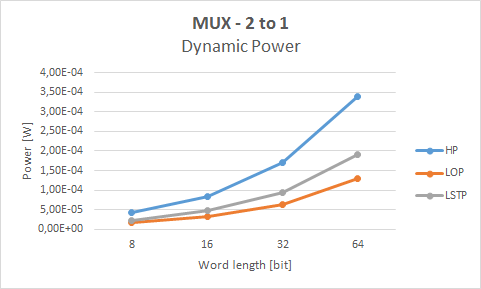
\includegraphics[scale=0.8]{immagini/2to1D}
	\caption{\textit{}} 
	\label{1}
\end{figure}
\newpage
\begin{figure}[!h]
	\centering
	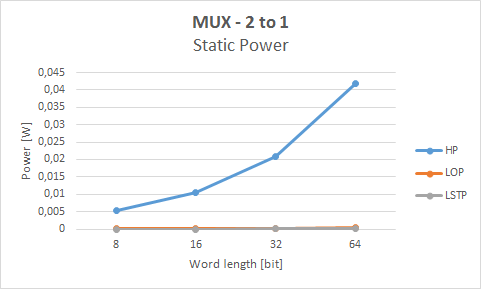
\includegraphics[scale=0.8]{immagini/2to1S}
	\caption{\textit{}} 
	\label{2}
\end{figure}

\begin{figure}[!h]
	\centering
	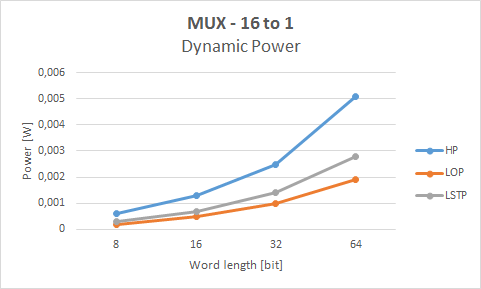
\includegraphics[scale=0.8]{immagini/16to1D}
	\caption{\textit{}} 
	\label{3}
\end{figure}

\begin{figure}[!h]
	\centering
	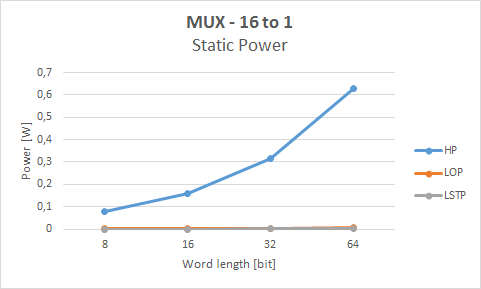
\includegraphics[scale=0.8]{immagini/16to1S}
	\caption{\textit{}} 
	\label{4}
\end{figure}
\newpage
\begin{figure}[!h]
	\centering
	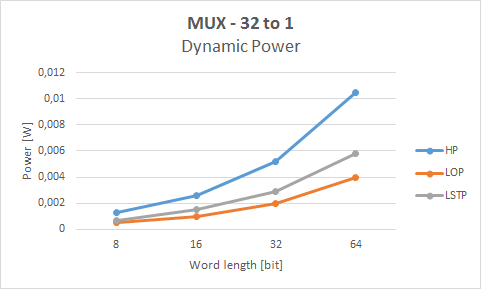
\includegraphics[scale=0.8]{immagini/32to1D}
	\caption{\textit{}} 
	\label{5}
\end{figure}

\begin{figure}[!h]
	\centering
	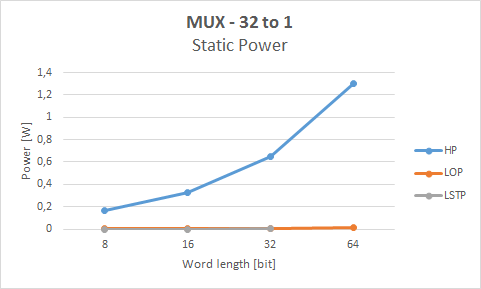
\includegraphics[scale=0.8]{immagini/32to1S}
	\caption{\textit{}} 
	\label{6}
\end{figure}

\begin{figure}[!h]
	\centering
	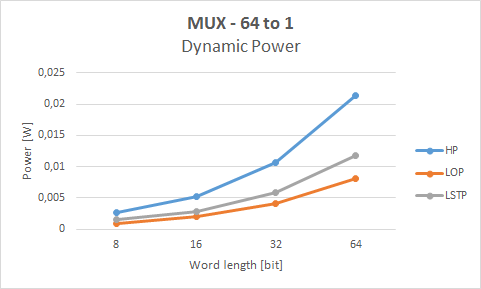
\includegraphics[scale=0.8]{immagini/64to1D}
	\caption{\textit{}} 
	\label{7}
\end{figure}
\newpage
\begin{figure}[!h]
	\centering
	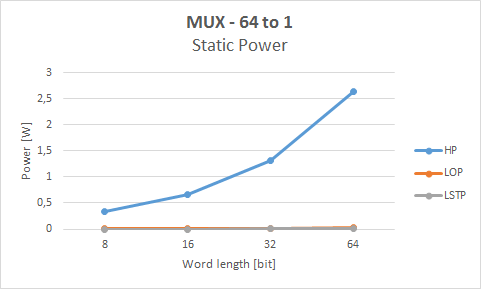
\includegraphics[scale=0.8]{immagini/64to1S}
	\caption{\textit{}} 
	\label{8}
\end{figure}

\begin{figure}[!h]
	\centering
	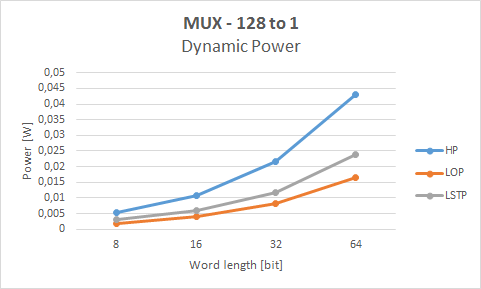
\includegraphics[scale=0.8]{immagini/128to1D}
	\caption{\textit{}} 
	\label{9}
\end{figure}

\begin{figure}[!h]
	\centering
	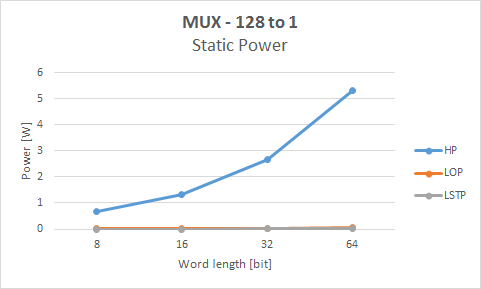
\includegraphics[scale=0.8]{immagini/128to1S}
	\caption{\textit{}} 
	\label{10}
\end{figure}
\newpage
%---------------------------------------------------------------
%	CODICE
%---------------------------------------------------------------
\section{Matlab implementation}
In the table below are reported the input data.

\begin{table}[h]
	\begin{center}
		\begin{tabular}{|c|c|c|c|} \hline
			\textbf{Quantity name} & \textbf{Description} & \textbf{u.m. (S.I.)} & \textbf{Variable name} \\ \hline
			$X$ &Number of input (is a power of 2) & / & X \\ 
			$W$ &Parallelism (is a power of 2) & / & Word \\
			$P_{static} NAND FO1$ &Static power NAND FO1 & W & P\_stat\_FO1 \\ 
			$P_{static} NAND FO2$ &Static power NAND FO2 & W & P\_stat\_FO2 \\ 
			$P_{static} NAND FO4$ &Static power NAND FO4 & W & P\_stat\_FO4 \\ 
			$P_{dyn} NAND FO1$ &Dynamic power NAND FO1 & W & P\_dyn\_FO1 \\ 
			$P_{dyn} NAND FO2$ &Dynamic power NAND FO2 & W & P\_dyn\_FO2 \\ 
			$P_{dyn} NAND FO4$ &Dynamic power NAND FO4 & W & P\_dyn\_FO4 \\  \hline 
		\end{tabular}
	\end{center}
	\caption{Input data}
	\label{tab1}
\end{table}

In the table below are reported the output data.

\begin{table}[h]
	\begin{center}
		\begin{tabular}{|c|c|c|c|} \hline
			\textbf{Quantity name} & \textbf{Description} & \textbf{u.m. (S.I.)} & \textbf{Variable name} \\ \hline
			$P_{static}$ &Static power MUX & W & P\_stat \\ 
			$P_{dynamic}$ &Dynamic power MUX & W & P\_dyn \\ \hline 
		\end{tabular}
	\end{center}
	\caption{Input data}
	\label{tab1}
\end{table}

\subsection{Main code}
The program asks the user to select the technology workspace needed and requires to specify the number of inputs and the parallelism of the MUX. The programs needs that both number of inputs and parallelism are power of two.
	\lstinputlisting{capitoli/code/main_mux_power.m}	
	
%\end{titlepage}

